\section{Data}
\label{sec:data}
\subsection{DR9 LRGs}
Luminous red galaxies (LRGs) are massive galaxies that lack active star formation and considered as one of the highly biased tracers of large scale structure. Redshift of LRGs can be easily determined from  a break around 4000 \AA~in their spectra. LRGs are widely targeted in previous galaxy redshift surveys \mr{(see, e.g., Eisenstein et al 2001, Prakash et al 2016)}, and their clustering and redshift properties are well studied \mr{(see, e.g., Reid et al 2016)}. DESI is expected to collect spectra of millions of LRGs covering the redshift range of $0.4<z<1.0$ over the span of its five year mission. Targets for DESI spectroscopy are selected from imaging surveys conducted from the Blanco telescope at Cerre-tololo in Chile and Bok and Mayall telescopes at Kitt Peak in Arizona, USA.


\begin{table*}
    \caption{Selection criteria for the DESI-like LRG targets from \mr{Zhou et al (2022)}.}
    \label{tab:ts}
    \centerline{%
    \begin{tabular}{lll}
    \hline
    \hline
     \textbf{Footprint} & \textbf{Criterion} &\textbf{Description}\\
      \hline
      \hline   
    &  $z_{\rm fiber} < 21.7$  & Faint limit  \\
          DECaLS & $z - W1 > 0.8 \times (r - z) - 0.6$ & Stellar rejection  \\
     & $[(g-r >1.3)~{\rm AND}~((g-r) > -1.55*(r-W1) + 3.13)]~{\rm OR}~(r -W 1 > 1.8)$ & Remove low-z galaxies \\
     & $[(r-W1 > (W1 - 17.26)*1.8)~{\rm AND}~(r - W1 > W1 - 16.36)]~{\rm OR}~(r-W1 > 3.29)$ & Luminosity cut \\ 
    \hline
    & $z_{\rm fiber} < 21.71$  & Faint limit  \\
 BASS+MzLS    & $z - W1 > 0.8 \times (r - z) - 0.6$ & Stellar rejection  \\
    & $[(g-r >1.34)~{\rm AND}~((g-r) > -1.55*(r-W1) + 3.23)]~{\rm OR}~(r -W 1 > 1.8)$ & Remove low-z galaxies \\
    & $[(r-W1 > (W1 - 17.24)*1.83)~{\rm AND}~(r - W1 > W1 - 16.33)]~{\rm OR}~(r-W1 > 3.39)$ & Luminosity cut \\ 
      \hline
      \end{tabular}
      }
\end{table*}

\begin{figure}
    \centering
    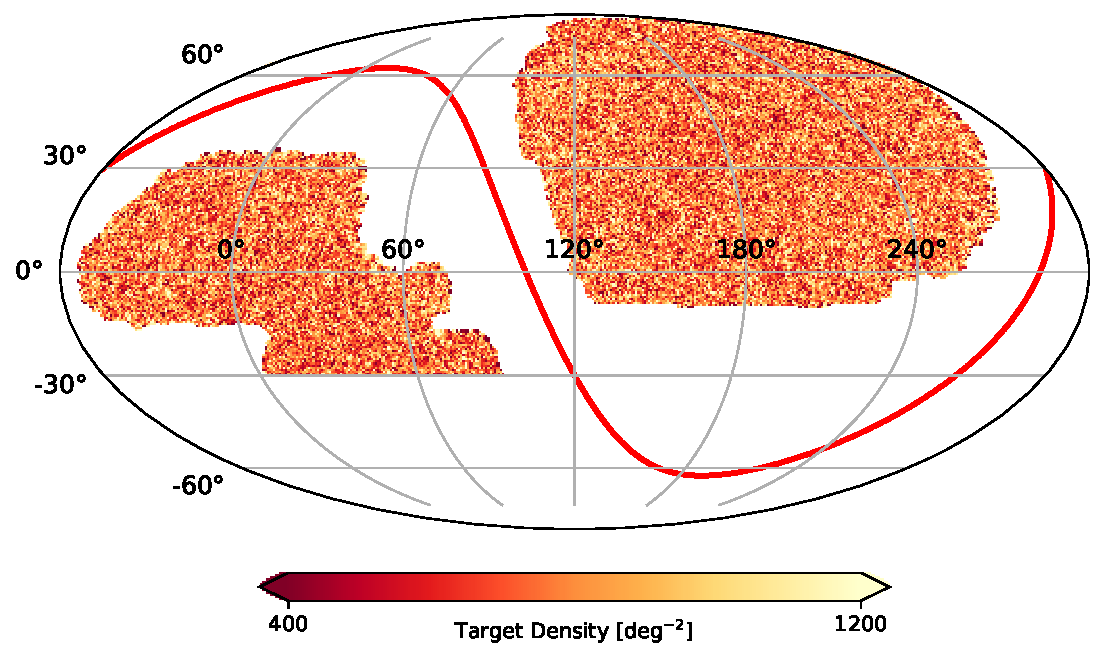
\includegraphics[width=0.45\textwidth]{figures/lrgdens.pdf}
    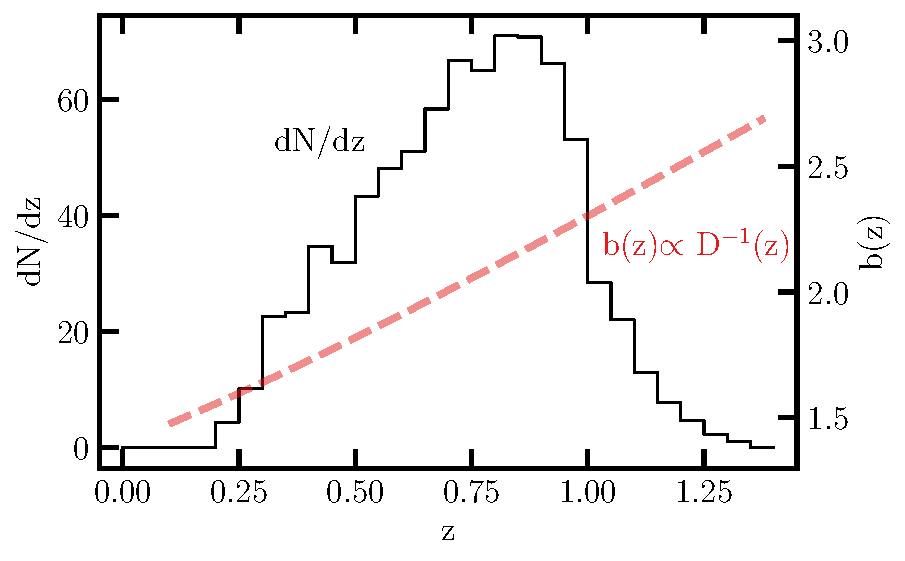
\includegraphics[width=0.45\textwidth]{figures/nz_lrg.pdf}
    \caption{Top: Observed density field of DESI Luminous Red Galaxies Data Release 9 \mr{(Dey et al 2018)} in deg$^{-2}$ . Spurious disconnected islands from the DECaLS North footprint at Declination below $-11$ and parts of the DECaLS South with Declination below $-30$ are dropped from the DR9 sample due to potential calibration issues. Bottom: Redshift distribution and bias evolution of DESI LRGs \mr{(Zhou et al 2021, Zhou et al 2022, Dawson et al 2022)}. The redshift distribution is deducted from spectroscopy and the bias model assumes a constant clustering amplitude.}
    \label{fig:ng}
\end{figure}


We use photometric LRGs selected from the DESI Imaging Surveys Data Release 9 \citep[DR9;][]{dey2018overview} using the selection designed for the DESI 1\% survey \mr{(Dawson et al 2022)}, described as SV3 in \cite{zhou2021clustering}. The color-magnitude cuts are described in the $g$, $r$, $z$ bands in the optical and $W1$ band in the infrared, and summarized here in Tab. \ref{tab:ts}. The implementation of these selections in the DESI pipeline is described in \mr{Myers et al (2022)}. DESI-like LRGs are selected brighter than the survey depth limits, and thus the sample density field is nearly homogenous. To further reduce stellar contamination, the sample is masked for bright stars, foreground bright galaxies as well as clusters of galaxies \footnote{See the maskbits at \url{https://www.legacysurvey.org/dr9/bitmasks/}}. Then, it is binned into \textsc{healpix} \citep{gorski2005healpix} at $\textsc{nside}=256$ to construct the density map with an average density of $800$ deg$^{-2}$ with a coverage around \mr{$14,000$} square degrees of the sky. The density map is corrected for pixel incompleteness in the density field of LRGS using a catalog of random points, uniformly scattered over the footprint with the same cuts and masks applied to the DR9 LRGs. Fig. \ref{fig:ng} (top) shows observed density field of DR9 LRGs in deg$^{-2}$. There are some disconnected islands, hereafter referred to as \textit{spurious islands}, in the DECaLS North region at Declination below $-11$, which are removed from the sample to minimize potential calibration issues. Additionally, parts of the DECaLS South with Declination below $-30$ are cut from the sample, since similar calibration issues might tamper with our analysis. We present  how these data cuts influence our $\fnl$ constraints in Section \ref{sec:results}. Fig. \ref{fig:ng} (bottom) illustrates the redshift distribution of our sample which is inferred from the DESI Survey Validation data \mr{(Dawson et al 2022)}, and the evolution of  galaxy bias for our LRG sample adapted from \cite{zhou2021clustering}, consistent with the assumption of a constant clustering amplitude.

\subsection{Lognormal Simulations}
\textsc{FLASK} (Full-sky Lognormal Astro-fields Simulation Kit; \mr{Xavier et al. 2016}) is used to generate two series of $1000$ galaxy density maps with $\fnl=0$ and $76.92$ using $b(z)=1.43/D(z)$. The fiducial cosmology to generate the mocks is based on,
\begin{equation*}
h = 0.67, \Omega_{b}=0.048, \Omega_{cdm}=0.264, \sigma_{8}=0.8225, {\rm and}~ n_{s}=0.9667.
\end{equation*}



\subsection{Imaging Templates}
We study the correlation coefficient between the LRG density map and potential sources of systematic error, mapped into \textsc{healpix} at the same \textsc{nside}. The maps used in this work are local stellar density constructed from point-like sources with a g-band magnitude in the range $12 \leq g < 17$ from Gaia Data Release 2 \citep[see,][]{gaiadr2, myers2022},  Galactic extinction E[B-V] from \cite{schlegel1998maps}, and other imaging properties including survey depth (galaxy depth in grz and PSF depth in W1) and seeing in grz from DESI imaging. Fig. \ref{fig:pcc} shows the Spearman correlation between galaxy density and imaging properties.

\begin{figure}
    \centering
    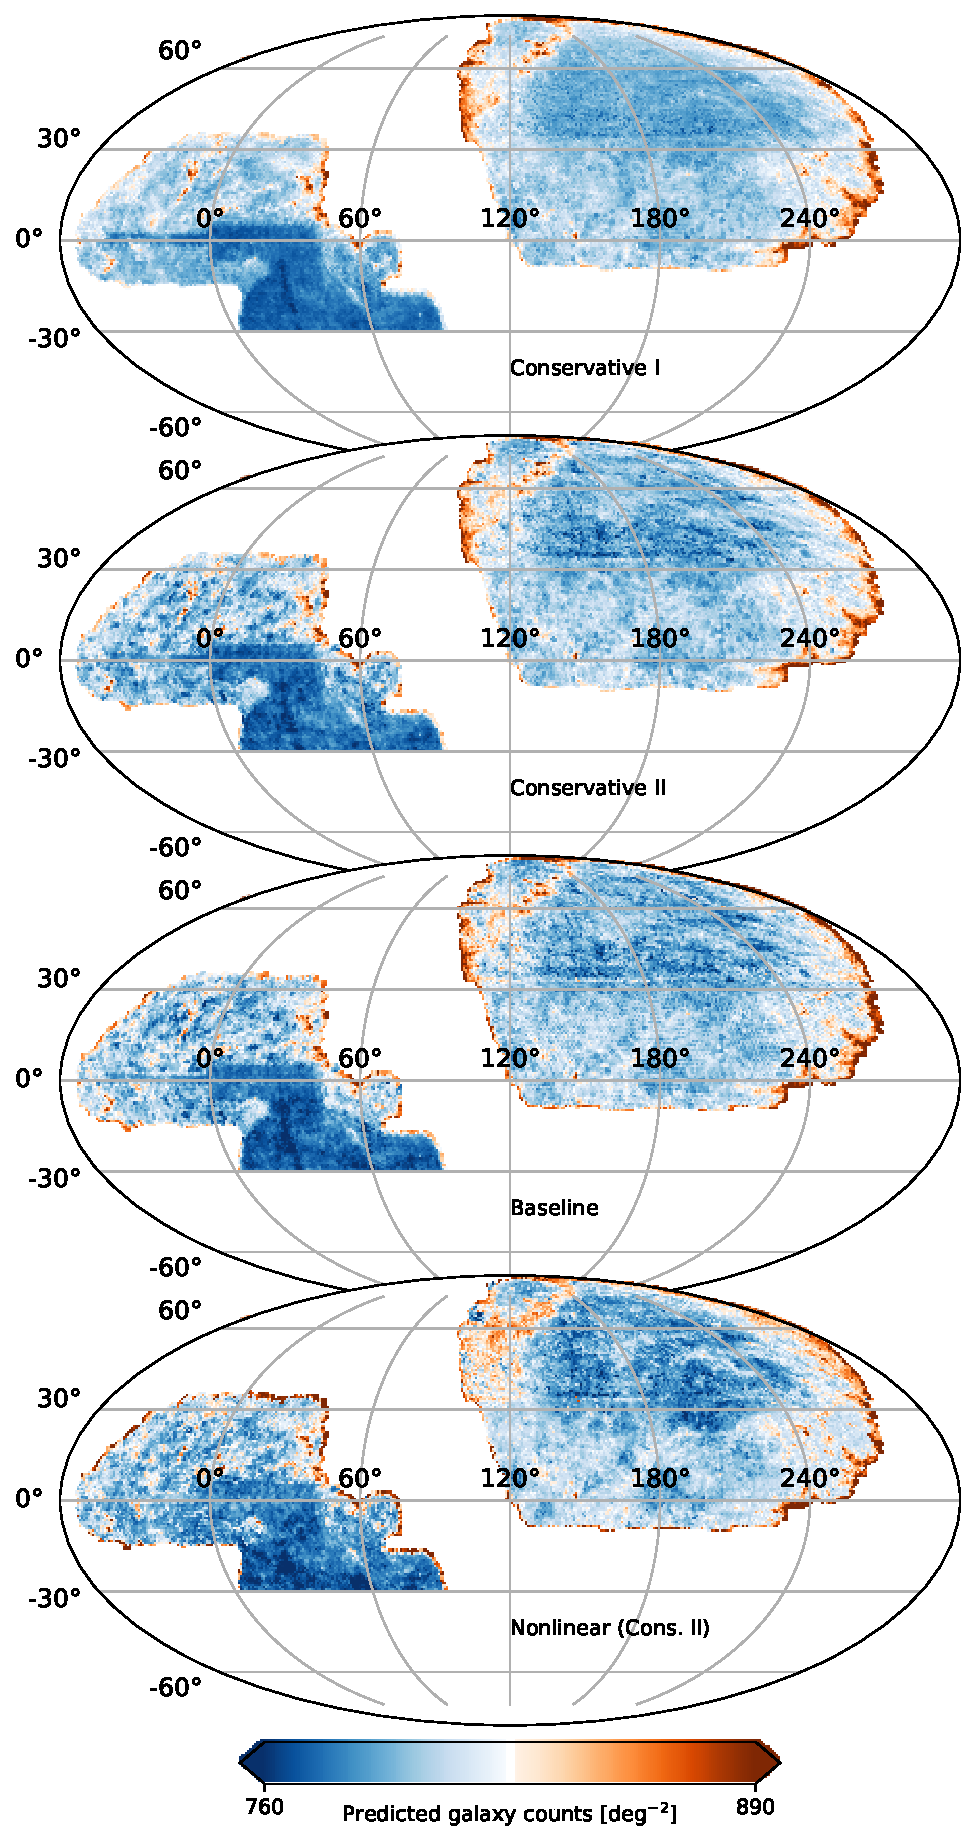
\includegraphics[width=0.45\textwidth]{figures/npred.pdf}
    \caption{Predicted galaxy counts from template regression. Baseline approach uses imaging maps from Zhou et al. (2022): EBV, galaxy depth in rgz, psfdepth in W1, and psfsize in grz. Conservative I uses EBV and galaxy depth in z, and Conservative II uses EBV, galaxy depth in z, and psfsize in r. In all approaches, the models are regressed on BASS+MzLS, DECaLS North, and DECaLS South separately.}
    \label{fig:npred}
\end{figure}

\begin{figure}
    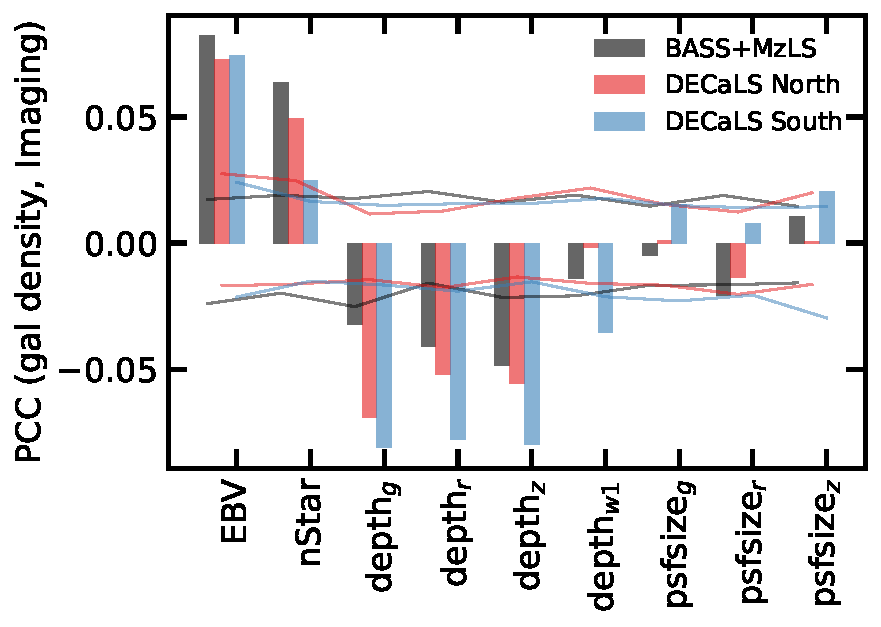
\includegraphics[width=0.45\textwidth]{figures/pcc.pdf} 
    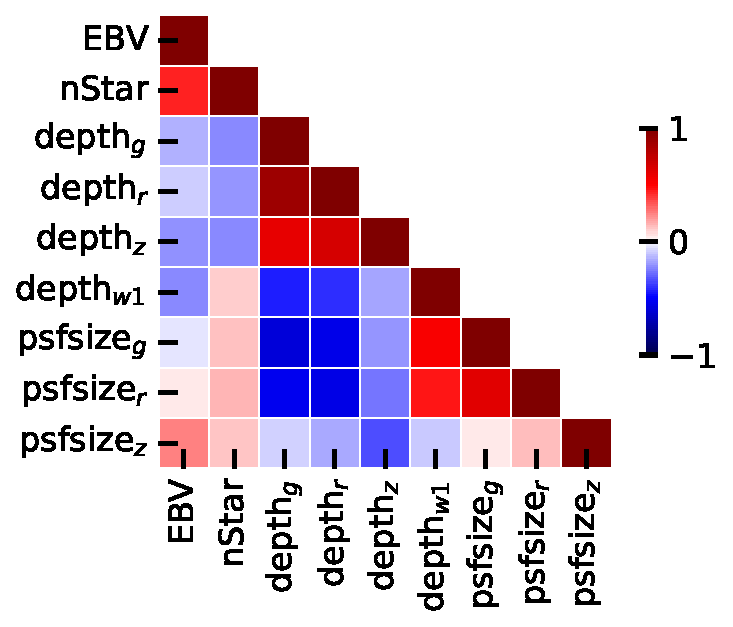
\includegraphics[width=0.45\textwidth]{figures/pccx.pdf}     
    \caption{Top: Pearson-r correlation coefficient between galaxy density and imaging properties in the three imaging regions (top) and between imaging properties themselves for the full DESI footprint (bottom). Solid curves represent the range of correlations observed in 100 randomly selected mock realizations.}
    \label{fig:pcc}
\end{figure}
